\chapter{电荷、电流与导电}\label{ch:b2:charges-currents-conduction}

合上开关，灯立刻亮起；然而铜线中的电子
朝灯的方向漂移，速度只有每秒零点几毫米，
要走上好几个小时才能到达。一道闪电携带三万
安培的电流，通过的通道只有手指粗细；驱动这根手指的神经
中流过的电流只有皮安量级。本科一年级分册把
电流当作导线中的数值，$I = U/R$；本章则把它们描述为
一个\emph{场}——物质中每一点处都有\omterm{def:b2:charges-currents-conduction:densities}{电流密度}——并写出
电荷永不产生也不消失的守恒律，并由
金属中电子的无规碰撞导出欧姆定律——这正是
电阻器、保险丝和霍尔传感器背后的微观图像。

\begin{omfigure}
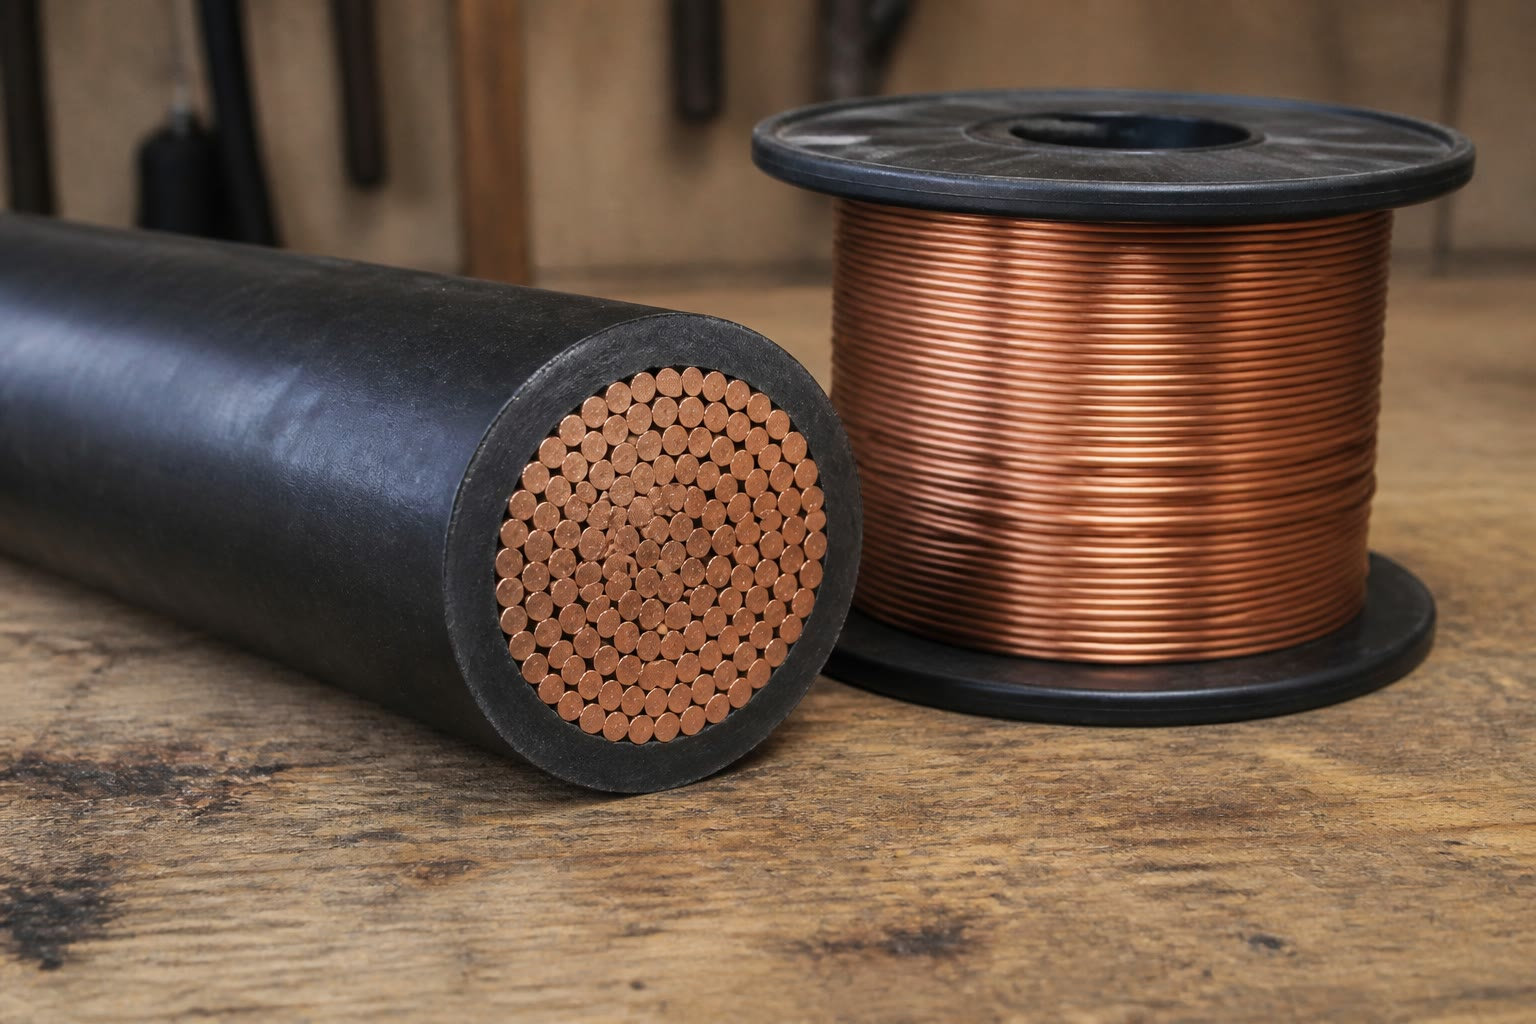
\includegraphics[width=0.58\linewidth]{images/book4/ai/b4-10-copper-wire-cable.jpg}

{\small 铜，电气世界的导体：这根电缆的导线中，每立方米约有 $10^{29}$ 个电子，以每秒不到一毫米的速度漂移。}
\end{omfigure}


\section{电荷与电流密度}

\begin{definition}[电荷密度；电流密度]\label{def:b2:charges-currents-conduction:densities}
\index{电荷密度}\index{电流密度}\index{电流强度}
在\omterm{def:b2:fluid-kinematics:particle}{介观尺度}上，物质带有\emph{体电荷密度}
$\rho(M, t)$（\unit{C/m^3}）：$\rho\,\dd\tau$ 为 $\dd\tau$ 中的电荷。曲面
可带有\emph{面电荷密度} $\sigma$（\unit{C/m^2}），导线带有线
电荷密度 $\lambda$（\unit{C/m}）。若第 $i$ 种载流子（电荷
$q_i$，数密度为 $n_i$）以平均速度 $\vect v_i$ 运动，则
\emph{电流密度}为
\[
\vect j = \sum_in_iq_i\,\vect v_i \qquad (\unit{A/m^2}) ,
\]
而通过有向曲面 $S$ 的\emph{电流强度}为其通量
$I = \iint_S\vect j\cdot\vect n\,\dd S$，即单位时间内穿过 $S$ 的
电荷量。对于单一种载流子，$\vect j = \rho_m\vect v$，其中 $\rho_m = nq$ 为
可动电荷的密度。
\end{definition}

\begin{proof}
在 $\dd t$ 时间内，第 $i$ 种载流子中穿过 $\dd S$ 的，
即位于以 $\dd S$ 为底、母线为 $\vect v_i\dd t$ 的斜柱体内者，其数目为
$n_i\vect v_i\cdot\vect n\,\dd S\,\dd t$，电荷量为其乘以 $q_i$。
\end{proof}

\begin{example}[电子漂移有多慢]\label{ex:b2:charges-currents-conduction:drift}
\index{漂移速度}
铜每个原子提供一个传导电子：$n = \rho_{\text{Cu}}N_A/M =
8900 \times 6.02 \times 10^{23}/0.0635 = \qty{8.5e28}{m^{-3}}$。在截面积为
\qty{1.5}{mm^2} 的导线中通以 \qty{10}{A} 的电流时，$j = \qty{6.7e6}{A/m^2}$，而
\emph{\omterm{ex:b2:charges-currents-conduction:drift}{漂移速度}}为 $v = j/ne = 6.7 \times 10^6/(8.5 \times 10^{28} \times 1.6 \times
10^{-19}) = \qty{0.5}{mm/s}$——每米需两个小时。灯之所以
立刻亮起，是因为推动电子的\emph{场}
在纳秒量级内就沿整根导线建立起来（它以接近光速传播，
如\cref{ch:b2:dispersion-wave-packets}中的电缆所示）：
所有电子同时开始运动，如同满管的水，一经推动便一齐流出。
\end{example}

\begin{omfigure}
\begin{tikzpicture}[font=\small, x=1cm, y=1cm, >=Stealth]
  \begin{scope}
    \draw[thick, omDef] (-2.6,0.7) .. controls (-1,0.9) and (0.5,0.3) .. (2.6,0.5);
    \draw[thick, omDef] (-2.6,-0.7) .. controls (-1,-0.9) and (0.5,-0.3) .. (2.6,-0.5);
    \draw[thick, omDef] (-2.6,0) ellipse (0.2 and 0.7); \draw[thick, omDef] (2.6,0) ellipse (0.15 and 0.5);
    \foreach \y in {-0.4,0,0.4} \draw[omThm, thick, ->] (-1.6,{\y*1.1}) -- (-0.6,{\y*0.9});
    \foreach \y in {-0.3,0,0.3} \draw[omThm, thick, ->] (0.8,{\y*0.9}) -- (1.9,{\y*0.8});
    \node[omThm, font=\footnotesize] at (-1.1,1.25) {$\vect j$};
    \node[font=\footnotesize] at (0,-1.4) {电流管：$I = \iint\vect j\cdot\vect n\,\dd S$ 各截面相同};
  \end{scope}
  \begin{scope}[xshift=8.0cm]
    \draw[thick, fill=omDef!10] (-2.2,-0.8) rectangle (2.2,0.8);
    \foreach \x/\y in {-1.6/0.4,-0.9/-0.3,-0.2/0.5,0.5/-0.5,1.2/0.3,1.7/-0.2} \fill (\x,\y) circle (1.4pt);
    \draw[omThm, ->] (-1.6,0.4) -- (-1.2,0.1) -- (-1.35,-0.35) -- (-0.8,-0.2) -- (-0.5,0.25);
    \draw[omDef, very thick, ->] (-0.3,-1.15) -- (1.2,-1.15) node[right, font=\footnotesize] {$\vect v$（漂移）};
    \draw[omProp, very thick, ->] (1.2,1.15) -- (-0.3,1.15) node[left, font=\footnotesize] {$\vect E$};
    \node[font=\footnotesize] at (0,-1.6) {};
  \end{scope}
\end{tikzpicture}

{\small 左：一根电流管——稳恒状态下，
每个截面通过的\omterm{def:b2:charges-currents-conduction:densities}{电流强度}相同。右：金属中的一个电子在两次碰撞之间折线运动，速率约为
$10^6$ m/s；电场使其叠加一个缓慢的漂移，
方向与 $\vect E$ 相反，速度为每秒不到一毫米。}
\end{omfigure}

\begin{example}[数量级]\label{ex:b2:charges-currents-conduction:orders}
闪电，电流为 \qty{30}{kA}，通道半径为 \qty{1}{cm}，则 $j \approx \qty{1e8}{A/m^2}$。
家用导线：$10^6$--$10^7$。阴极射线管中的电子束，
\qty{1}{mA} 流经 \qty{1}{mm^2}：$10^3$。神经纤维，\qty{1}{nA} 通过
\qty{10}{\micro m^2}：$10^2$。粒子加速器中的束流，\qty{1}{A} 通过
\qty{0.1}{mm^2} 的光斑：$10^7$——且在真空中，完全没有碰撞。
\end{example}

\section{电荷守恒}

\begin{theorem}[电荷的局域守恒]\label{thm:b2:charges-currents-conduction:conservation}
\index{电荷的局域守恒}\index{连续性方程（电荷）}
在每一点处，
\[
\frac{\partial\rho}{\partial t} + \operatorname{div}\vect j = 0 ;
\]
对固定体积 $V$ 积分，其边界为闭曲面 $\Sigma$，
$\dd Q_V/\dd t = -I_{\text{流出}}$：体内电荷的改变只取决于
穿过边界的电荷。在\emph{稳恒状态}（$\partial_t\rho = 0$）下，
$\operatorname{div}\vect j = 0$：$\vect j$ 的通量沿电流管守恒，
同一\omterm{def:b2:charges-currents-conduction:densities}{电流强度}穿过导线的每个截面，并且
流入节点的电流等于流出的电流（基尔霍夫节点定律）。
\end{theorem}

\begin{proof}
逐字照搬\cref{thm:b2:fluid-kinematics:continuity}中的质量守恒关系，
其中 $\rho$ 为\omterm{def:b2:charges-currents-conduction:densities}{电荷密度}，$\vect j$ 为对应的\omterm{def:b2:charges-currents-conduction:densities}{电流密度}：
单位体积内，通过固定小盒六个面的电荷净流出量为
$\operatorname{div}\vect j$，且没有电荷被产生。积分形式
对各小盒求和（内部各面相互抵消）。对于两截面
$S_1$、$S_2$ 之间侧面无通量的电流管，有 $I_1 = I_2$；节点是
接有若干导线的小体积：$\sum I_{\text{流入}} = \sum I_{\text{流出}}$。
\end{proof}

\begin{remark}[电流中断之处：电容器]\label{rem:b2:charges-currents-conduction:capacitor}
向电容器极板供电的导线是一段会中断的电流管：
流入极板的 $\vect j$ 通量为 $I = \dd Q/\dd t$，电荷在极板上积累
——此处 $\operatorname{div}\vect j \ne 0$，流动不是稳恒的。
然而另一侧导线中的电流同样为 $I$：必须有某物
跨越间隙承担这一平衡。在\cref{ch:b2:maxwell-equations}中
它被命名为——位移电流——，并使电荷守恒
成为麦克斯韦方程组的基石。
\end{remark}

\section{德鲁德模型与欧姆定律}

\begin{proposition}[德鲁德模型；局域欧姆定律]\label{prop:b2:charges-currents-conduction:drude}
\index{德鲁德模型}\index{局域欧姆定律}\index{电导率}\index{电阻率}\index{迁移率}
设金属中的导电电子为自由粒子（质量 $m$，
电荷 $-e$、数密度 $n$），它们受电场 $\vect E$ 作用，
并平均每隔 $\tau$ 秒与晶格碰撞一次，从而失去漂移动量
——对平均速度相当于摩擦力 $-m\vect v/\tau$：
\[
m\frac{\dd\vect v}{\dd t} = -e\vect E - \frac m\tau\vect v .
\]
稳恒场中，\omterm{ex:b2:charges-currents-conduction:drift}{漂移速度}在数个 $\tau$ 内趋于 $\vect v = -e\tau
\vect E/m$，\omterm{def:b2:charges-currents-conduction:densities}{电流密度}为
\[
\vect j = \gamma\,\vect E , \qquad \gamma = \frac{ne^2\tau}{m} :
\]
即\emph{局域欧姆定律}，其中 $\gamma$ 为\emph{电导率}
（\unit{S/m}；其倒数 $\rho_e = 1/\gamma$ 为\emph{电阻率}，
\unit{\ohm.m}）。漂移速率与场强之比 $\mu = e\tau/m$ 称为
\emph{迁移率}（\unit{m^2/(V.s)}）。对长为 $L$、
截面面积为 $S$ 且均匀的导体，通以均匀的 $\vect j$，沿长度对 $E = j/\gamma$
积分，得 $U = EL = (L/\gamma S)I$，电阻为 $R = L/\gamma S
= \rho_eL/S$，即本科一年级分册中的电阻公式。
\end{proposition}

\begin{proof}
由 $\vect v = -e\tau\vect E/m$ 得 $\vect j = -ne\vect v = (ne^2\tau/m)\vect E$。
瞬态 $\vect v(t) = \vect v_\infty(1 - \eu^{-t/\tau})$ 的持续时间为 $\tau \sim
\qty{1e-14}{s}$，相对于任何电路的时间尺度都是瞬时的。
电阻由两端之间的 $\int\vect E\cdot\dd\vect l$ 得出。
\end{proof}

\begin{example}[铜，由实测电导率求得]\label{ex:b2:charges-currents-conduction:copper}
铜：$\gamma = \qty{6.0e7}{S/m}$，$n = \qty{8.5e28}{m^{-3}}$：$\tau = m\gamma/ne^2 =
9.1 \times 10^{-31} \times 6 \times 10^7/(8.5 \times 10^{28} \times 2.56 \times 10^{-38}) = \qty{2.5e-14}{s}$
——两次碰撞之间相隔 25 飞秒。金属中电子的
无规速率约为 \qty{1.6e6}{m/s}（这是量子效应，而非
热运动 $\sqrt{3k_BT/m} \approx \qty{1e5}{m/s}$），因此平均自由程为 $\ell
= v\tau \approx \qty{40}{nm}$，约为 100 个原子间距：电子并不
与原子本身碰撞（完美晶体对它们是透明的），而是与
其中的缺陷和热振动碰撞——这正是
金属被加热或合金化时 $\gamma$ 下降的原因。迁移率 $e\tau/m =
\qty{4.4e-3}{m^2/(V.s)}$：相当于每伏特每米 \qty{4}{mm/s}。
\end{example}

\begin{proposition}[高频下的欧姆定律]\label{prop:b2:charges-currents-conduction:acdrude}
\index{复电导率}
对正弦场 $\underline{\vect E}\,\eu^{\iu\omega t}$，德鲁德方程
给出 $\underline{\vect j} = \underline\gamma(\omega)\underline{\vect E}$，其中
\[
\underline\gamma(\omega) = \frac{\gamma_0}{1 + \iu\omega\tau} , \qquad \gamma_0 = \frac{ne^2\tau}{m} :
\]
电导率为实数，且在 $\omega\tau
\ll 1$ 时等于其直流值，即对铜直至约 \qty{1e13}{Hz}，贯穿
整个无线电与微波波段；在红外线与可见光（$\omega\tau \gg 1$）时
它变为纯虚数，$\underline\gamma \approx ne^2/\iu m\omega$：电子
自由振荡，与场异相，金属的行为
与\cref{ch:b2:waves-in-media}中的等离子体相同。
\end{proposition}

\begin{proof}
$\iu\omega m\underline{\vect v} = -e\underline{\vect E} - m\underline{\vect v}/\tau$，由此
可得 $\underline{\vect v} = -e\tau\underline{\vect E}/m(1 + \iu\omega\tau)$，且 $\underline{\vect j}
= -ne\underline{\vect v}$。
\end{proof}

\begin{omfigure}
\begin{tikzpicture}
\begin{axis}[omaxis, axis x line=bottom, axis y line=left, width=7.6cm, height=4.6cm,
    xmode=log, xmin=0.01, xmax=100, ymin=0, ymax=1.1, xlabel={$\omega\tau$}, ylabel={$\underline\gamma/\gamma_0$},
    xtick={0.01,0.1,1,10,100}, ytick={0,0.5,1}, samples=200,
    xlabel style={at={(axis description cs:0.5,-0.2)}, anchor=north},
    ylabel style={at={(axis description cs:-0.12,0.5)}, rotate=90, anchor=south},
    legend style={font=\scriptsize, at={(0.97,0.95)}, anchor=north east, draw=none, fill=none}]
  \addplot[omThm, thick, domain=0.01:100] {1/(1+x*x)};
  \addplot[omDef, thick, domain=0.01:100] {x/(1+x*x)};
  \legend{$\operatorname{Re}$, $-\operatorname{Im}$}
\end{axis}
\end{tikzpicture}
\hfill
\begin{tikzpicture}[font=\small, x=1cm, y=1cm, >=Stealth]
  \draw[thick, fill=omExo!15] (-2.2,-0.6) rectangle (2.2,0.6);
  \draw[omThm, very thick, ->] (-3.0,0) -- (-2.25,0) node[above, pos=0.3, font=\footnotesize] {$I$};
  \draw[omThm, very thick, ->] (2.25,0) -- (3.0,0);
  \foreach \x in {-1.5,-0.5,0.5,1.5} \node[omProp, font=\footnotesize] at (\x,0.0) {$\otimes$};
  \node[omProp, font=\footnotesize] at (1.5,0.95) {$\vect B$};
  \draw[omDef, thick, ->] (0,0.25) -- (0,-0.4) node[right, font=\footnotesize, pos=0.5] {$\vect E_H$};
  \fill[omDef] (-0.6,0.6) circle (1.3pt); \fill[omDef] (-0.6,-0.6) circle (1.3pt);
  \node[omDef, font=\footnotesize] at (-0.9,0.85) {$+$}; \node[omDef, font=\footnotesize] at (-0.9,-0.85) {$-$};
  \node[font=\footnotesize] at (0,-1.3) {$\vect E_H = -\dfrac1{nq}\,\vect j\wedge\vect B$};
\end{tikzpicture}

{\small 左图：德鲁德电导率随 $\omega\tau$ 的变化——低频时为实的常数，
超过 $1/\tau$ 后变为纯虚数。右图：导体条中的霍尔
效应——载流子在场的作用下被推向侧面，
使边缘带电，横向霍尔场与
磁力相平衡。}
\end{omfigure}

\begin{remark}[导体、半导体、电解质]\label{rem:b2:charges-currents-conduction:materials}
\index{半导体}\index{电解质}
同一定律 $\vect j = \sum n_iq_i\mu_i\vect E$ 对所有导体均成立；
变化的是 $n$ 与 $\mu$。金属：$n \sim 10^{29}$，$\gamma \sim 10^7$
S/m。\omterm{rem:b2:charges-currents-conduction:materials}{半导体}：$n \sim 10^{16}$--$10^{23}$，由掺杂决定，
随温度急剧升高，并有两类载流子（电子与
空穴）——这正是热敏电阻与二极管的依据。\omterm{rem:b2:charges-currents-conduction:materials}{电解质}：正负两种离子，
$\mu \sim 10^{-8}$--$10^{-7}$ m$^2$/(V s)；海水 $\gamma \approx \qty{5}{S/m}$，
自来水 $10^{-2}$，纯水 $10^{-5}$。绝缘体（玻璃、聚合物）：
$\gamma \lesssim 10^{-12}$ S/m。本科一年级分册中的霍尔效应，以
局域形式 $\vect E_H = -\vect j\wedge\vect B/nq$ 表示，可测定 $n$ 及
$q$ 的符号。在铝和锌中，载流子竟为正——
即空穴——而经典模型对此无法解释。
\end{remark}

\section{能量：局部焦耳定律}

\begin{proposition}[局部焦耳定律]\label{prop:b2:charges-currents-conduction:joule}
\index{焦耳定律（局部形式）}
电场每单位体积、每单位时间传给载流子的功率
为 $\vect j\cdot\vect E$；在欧姆导体中，它为
\[
p = \vect j\cdot\vect E = \gamma E^2 = \frac{j^2}\gamma \ \ (\unit{W/m^3}) ,
\]
全部经碰撞转化为热量（漂移动能
可忽略且保持不变）。对整根导线积分，$\int j^2/\gamma\,\dd\tau
= (L/\gamma S)I^2 = RI^2$。
\end{proposition}

\begin{proof}
每个载流子所受的力 $q\vect E$ 做功的功率为 $q\vect E\cdot\vect v$；
对 $n\,\dd\tau$ 个载流子求和：$nq\vect v\cdot\vect E\,\dd\tau = \vect j\cdot
\vect E\,\dd\tau$（磁力不做功）。在\omterm{prop:b2:charges-currents-conduction:drude}{德鲁德模型}的稳态中，
此功率等于摩擦项耗散的功率，即
传递给晶格。
\end{proof}

\begin{example}[导线发热]\label{ex:b2:charges-currents-conduction:heating}
截面积为 \qty{1.5}{mm^2} 的导线，电流为 \qty{10}{A}：$p = j^2/\gamma = (6.7 \times 10^6)^2/6 \times 10^7 =
\qty{7.4e5}{W/m^3}$，即每米 \qty{1.1}{W}，很容易被
周围的空气带走。若无冷却，铜（$c = \qty{385}{J/(kg.K)}$，
$\rho = \qty{8900}{kg/m^3}$）的升温速率为 $p/\rho c = \qty{0.2}{K/s}$。若电流为 \qty{100}{A}，
同一导线中升温速率大百倍，即 \qty{20}{K/s}：约一分钟即
熔化——这正是保险丝的原理，其细导线
被设计为最先熔化。
\end{example}

\begin{proposition}[导体中电荷的弛豫]\label{prop:b2:charges-currents-conduction:relaxation}
\index{弛豫时间（导体）}
在欧姆导体中，体\omterm{def:b2:charges-currents-conduction:densities}{电荷密度}按 $\rho(t) =
\rho_0\eu^{-t/\tau_r}$ 衰减，其中
\[
\tau_r = \frac{\varepsilon_0}{\gamma} :
\]
对铜为 \qty{1.5e-19}{s}，对海水为 \qty{2e-12}{s}，对玻璃为 \qty{10}{s}。
在频率约为 $1/\tau_r$ 量级以内时，导体中\emph{不存在
体电荷}，任何多余的电荷都跑到表面。
因此，“导体”一词取决于时间尺度：海水对无线电波而言是导体，
对可见光而言则是绝缘体。
\end{proposition}

\begin{proof}
由电荷守恒、$\vect j = \gamma\vect E$ 及局部形式的高斯定理
$\operatorname{div}\vect E = \rho/\varepsilon_0$（见\cref{ch:b2:maxwell-equations}）可得：
$\partial_t\rho = -\gamma\operatorname{div}\vect E = -(\gamma/\varepsilon_0)\rho$。
\end{proof}

\begin{method}[由局部定律到积分定律]\label{met:b2:charges-currents-conduction:method}
求任意形状导体的电阻：(1) 利用
对称性写出 $\vect j$（稳恒时其通量守恒，
故在管状区域中 $j \times$ 截面积 $= I$）；(2) $\vect E = \vect j/\gamma$；(3) 沿
一条从一个电极到另一个电极的线对 $\vect E$ 积分：$U = \int\vect E\cdot
\dd\vect l$，且 $R = U/I$；(4) 用焦耳功率 $\int j^2/\gamma\,
\dd\tau = RI^2$ 校核。同样的步骤可用于求电缆的漏电、
避雷针周围大地的电阻，或锥形接触的电阻。
\end{method}

\section{练习}

\begin{exercise}[$\star$]\label{exo:b2:charges-currents-conduction:1}
截面积为 \qty{2.5}{mm^2} 的铜导线通有 \qty{16}{A} 的电流。求\omterm{def:b2:charges-currents-conduction:densities}{电流密度}、
漂移速率（$n = \qty{8.5e28}{m^{-3}}$）、电子沿导线走过
\qty{20}{m} 到达插座所需的时间；导线中的电场（$\gamma = \qty{6.0e7}{S/m}$）、
\qty{20}{m} 长度上的电压降以及损耗的功率。
\end{exercise}

\begin{exercise}[$\star$]\label{exo:b2:charges-currents-conduction:2}
求下列各情形的\omterm{def:b2:charges-currents-conduction:densities}{电流密度}：闪电放电（\qty{30}{kA}，半径 \qty{1}{cm}）；
电子束（\qty{2}{mA}，\qty{0.5}{mm^2}）；神经轴突（\qty{1}{nA}，半径
\qty{2}{\micro m}）；地球磁层环电流（\qty{1}{MA} 通过
约 \qty{1e14}{m^2}）。其中哪些超过上一题中的导线？
\end{exercise}

\begin{exercise}[$\star$]\label{exo:b2:charges-currents-conduction:3}
在 \qty{20}{\degreeCelsius} 时的电阻率：铜为 \qty{1.7e-8}{\ohm.m}，铝为
\qty{2.8e-8}{\ohm.m}，铁为 \qty{1.0e-7}{\ohm.m}，镍铬合金为 \qty{1.1e-6}{\ohm.m}。
求各材料制成的长 \qty{100}{m}、截面积为 \qty{2.5}{mm^2} 的导线的电阻；求与
\qty{2.5}{mm^2} 铜线等电阻的铝线的截面积，并求二者的质量之比（密度分别为
$8900$ 和 \qty{2700}{kg/m^3}）；求
功率为 \qty{1}{kW}、电压为 \qty{230}{V} 的电热器所用的 \qty{0.5}{mm} 镍铬合金丝的长度。
\end{exercise}

\begin{exercise}[$\star$]\label{exo:b2:charges-currents-conduction:4}
用\omterm{prop:b2:charges-currents-conduction:drude}{德鲁德模型}求 $\tau$、迁移率及平均自由程（随机速率为 \qty{1.6e6}{m/s}），
分别针对铜（$\gamma = \qty{6.0e7}{S/m}$，$n = \qty{8.5e28}{m^{-3}}$）和银
（$\gamma = \qty{6.3e7}{S/m}$，$n = \qty{5.9e28}{m^{-3}}$）；求
$n = \qty{1e22}{m^{-3}}$、$\mu = \qty{0.14}{m^2/(V.s)}$ 的硅样品的电导率；
求该样品在 \qty{1}{kV/m} 电场中的漂移速率。
\end{exercise}

\begin{exercise}[$\star\star$]\label{exo:b2:charges-currents-conduction:5}
一个极板面积为 $S$ 的电容器通过导线由电流 $I(t)$ 充电。(a) 对
包围一个极板的闭合曲面应用积分形式的守恒定律，
建立 $I$ 与极板电荷 $Q$ 的关系。(b) 为什么 $\operatorname{div}\vect j \ne 0$
在极板处？(c) 导电介质中半径为 $a$ 的球形电极
沿径向发出电流 $I$：求 $\vect j(r)$，并验证 $\operatorname{div}
\vect j = 0$（对 $r > a$，利用 $\operatorname{div}\vect j = \frac1{r^2}\partial_r(r^2j_r)$
对径向场计算）。(d) 那么，电荷守恒在何处
“失效”？
\end{exercise}

\begin{exercise}[$\star\star$]\label{exo:b2:charges-currents-conduction:6}
\emph{\omterm{prop:b2:dispersion-wave-packets:coax}{同轴电缆}的漏电。}两导体之间的绝缘体
（半径 $a = \qty{1}{mm}$，$b = \qty{3.5}{mm}$）的电导率为 $\gamma = \qty{1e-13}{S/m}$；
在两者之间加电压 $U$，有径向漏电流 $I$
沿长度 $L$ 流过。(a) 求 $\vect j(r)$ 与 $\vect E(r)$。(b) 证明
长度为 $L$ 的部分的电阻为 $R = \ln(b/a)/2\pi\gamma L$，求其每千米的
数值。(c) 在 \qty{1}{kV} 电压下，每千米的漏电流与功率。
(d) 将其与单位长度的电容 $2\pi\varepsilon_0\varepsilon_r/\ln(b/a)$ 比较：
证明 $RC = \varepsilon_0\varepsilon_r/\gamma$，并用弛豫时间解释之。
\end{exercise}

\begin{exercise}[$\star\star$]\label{exo:b2:charges-currents-conduction:7}
铜的\omterm{prop:b2:charges-currents-conduction:acdrude}{复电导率}（$\tau = \qty{2.5e-14}{s}$）。(a) 求 $\omega\tau$ 在
\qty{50}{Hz}、\qty{10}{GHz}（微波）、\qty{30}{THz}（红外线）、\qty{5e14}{Hz}
（绿光）。(b) 求 $\underline\gamma/\gamma_0$ 在各情形下的模与相位。
(c) 欧姆定律在 $1\%$ 精度内成立的频率上限是多少？(d) 在可见光范围内，
写出 $\underline\gamma$，并证明 $\underline{\vect j}$ 与
$\underline{\vect E}$ 相位正交；平均焦耳热功率是多少？
\end{exercise}

\begin{exercise}[$\star\star$]\label{exo:b2:charges-currents-conduction:8}
一根 \qty{0.20}{mm} 铜保险丝（铜：$\gamma = \qty{6.0e7}{S/m}$，$\rho =
\qty{8900}{kg/m^3}$，$c = \qty{385}{J/(kg.K)}$，在 \qty{1085}{\degreeCelsius} 熔化，
潜热为 \qty{205}{kJ/kg}）。(a) 求电流为 \qty{10}{A} 时单位体积的\omterm{def:b2:charges-currents-conduction:densities}{电流密度}与
焦耳热功率。(b) 求从 \qty{20}{\degreeCelsius} 加热至熔化所需的时间，
设无热量散失（忽略电阻率随温度的升高）。(c)
电流为 \qty{30}{A} 时同样求解。(d) 实际上，导线会向空气散热，这
如何决定保险丝的额定电流，以及为何将保险丝封装在
充砂的管壳之中？
\end{exercise}

\begin{exercise}[$\star\star$]\label{exo:b2:charges-currents-conduction:9}
\emph{弛豫。}(a) 由电荷守恒推导 $\partial_t\rho = -(\gamma/\varepsilon_0)\rho$，
结合欧姆定律与 $\operatorname{div}\vect E = \rho/\varepsilon_0$。(b)
求 $\tau_r$：铜、海水（$\gamma = \qty{5}{S/m}$）、自来水
（\qty{5e-2}{S/m}）、玻璃（\qty{1e-12}{S/m}）、聚四氟乙烯（\qty{1e-16}{S/m}）。(c)
各材料在多高频率下可视为“良导体”（电荷在一个
周期内弛豫）？(d) 一根带电玻璃棒可保持电荷数分钟，这是否
与前述结果相符？
\end{exercise}

\begin{exercise}[$\star\star\star$]\label{exo:b2:charges-currents-conduction:10}
\emph{接地。}一个半径为 $a = \qty{0.50}{m}$ 的半球形电极
与表面齐平地埋入电导率为 $\gamma =
\qty{0.010}{S/m}$ 的土壤中；电流 $I$ 由此流入，径向
扩散到半空间。(a) 求 $\vect j(r)$、$\vect E(r)$ 及电势 $V(r)$，取 $V(\infty) = 0$。
(b) 求接地电阻 $R = 1/2\pi\gamma a$ 并计算其值。(c) 一次
\qty{20}{kA} 的雷击击中接地棒，求棒的电势；
在 $r = \qty{10}{m}$ 与 \qty{10.7}{m} 处的电势；“跨步电压”即站在该处的人
两脚之间的电压（两脚相距 \qty{0.7}{m}，沿径向）。
(d) 为何四条腿相距较远的牛，
比人更常因附近雷击而死亡？
\end{exercise}

\begin{exercise}[$\star\star\star$]\label{exo:b2:charges-currents-conduction:11}
\emph{霍尔传感器。}厚度为 $t$、宽度为 $w$ 的薄片通有电流 $I$，
沿 $x$ 方向流动，磁场 $B$ 沿 $z$ 方向。(a) 由 $\vect E_H = -\vect j\wedge\vect B
/nq$，证明宽度两侧的霍尔电压为 $V_H = IB/nqt$。(b)
铜薄片，$t = \qty{0.10}{mm}$，\qty{1}{A}，\qty{1}{T}：求 $V_H$。(c) 一个掺杂
\omterm{rem:b2:charges-currents-conduction:materials}{半导体}，$n = \qty{1e22}{m^{-3}}$，几何尺寸相同：求 $V_H$；为何
传感器常用\omterm{rem:b2:charges-currents-conduction:materials}{半导体}。(d) 一个传感器，$n = \qty{1e22}{m^{-3}}$，$t =
\qty{20}{\micro m}$，通以 \qty{1}{mA} 的电流，读数为 \qty{10}{\micro V}，求所测磁场。
由 $V_H$ 的正负号能说明什么？
\end{exercise}

\begin{exercise}[$\star\star\star$]\label{exo:b2:charges-currents-conduction:12}
\emph{\omterm{rem:b2:charges-currents-conduction:materials}{电解质}。}在水中，Na$^+$ 与 Cl$^-$ 离子的迁移率为
$\mu_+ = \qty{5.2e-8}{m^2/(V.s)}$ 与 $\mu_- = \qty{7.9e-8}{m^2/(V.s)}$。(a)
证明 $\gamma = ne(\mu_+ + \mu_-)$，其中 $n$ 为
单位体积内的离子对数。(b) 海水含 \qty{0.5}{mol/L} 的 NaCl：求 $\gamma$，并与
实测值 \qty{5}{S/m} 比较。(c) 在 \qty{10}{V/m} 下的漂移速率；哪种离子
承载的电流更多？(d) 一段海水柱，截面 \qty{1}{cm^2}，长 \qty{10}{cm}，通有
\qty{1}{A} 的电流：求其电压、功率，以及将其升温 \qty{10}{K} 所需的时间（$c =
\qty{4.0}{kJ/(kg.K)}$）；为何电泳凝胶需要冷却。
\end{exercise}

\section{问题：铜导线，从原子到电网}

\begin{problem}[{周末问题——在四个尺度上考察一米长的家用导线：
电子、局域定律、电路与
输电线}]
\label{pb:b2:charges-currents-conduction:1}

铜：摩尔质量 \qty{63.5}{g/mol}，密度 \qty{8900}{kg/m^3}，每个原子
贡献一个传导电子，电导率 $\gamma = \qty{6.0e7}{S/m}$（
\qty{20}{\degreeCelsius} 时），电阻率随温度上升，$\rho_e(T) = \rho_e(20)[1 +
\alpha(T - 20)]$，其中 $\alpha = \qty{4.0e-3}{K^{-1}}$；$c = \qty{385}{J/(kg.K)}$。导线
截面 $S = \qty{2.5}{mm^2}$，长 \qty{1}{m}，电流 \qty{16}{A}。

\medskip
\noindent\textbf{第一部分——电子。}
\begin{enumerate}
  \item 传导电子的数密度 $n$。
  \item 求\omterm{def:b2:charges-currents-conduction:densities}{电流密度}与\omterm{ex:b2:charges-currents-conduction:drift}{漂移速度}；一个电子
        穿过这一米导线需要多长时间。
  \item 德鲁德的 $\tau$ 与迁移率；取随机速率 \qty{1.6e6}{m/s}，平均自由程
        约合多少个原子间距（\qty{0.26}{nm}）；
        这说明电子在与什么
        发生碰撞？
  \item 热振动随 $T$ 增大，因此粗略地有 $\tau \propto 1/T$：
        在室温附近与 $\alpha$ 比较（若 $\dd\rho_e/\rho_e =
        \dd T/T$ 则给出 $\alpha = 1/293$）。
  \item 导线中的电场；这一米导线两端的总电压；
        将每个电子的漂移动能与 $k_BT$ 比较——
        电子气是否因电流而受扰动？
  \item 每秒穿过导线任一截面的电子数。
  \item 这一米导线中传导电子的总电荷；
        电场作用于它们全体的合力；与
        导线的重力相比较。这个力最终去向何处（想想
        碰撞）？
\end{enumerate}

\medskip
\noindent\textbf{第二部分——局域定律。}
\begin{enumerate}[resume]
  \item 单位体积及单位长度的焦耳热功率。
  \item 导线置于空气中，单位表面以 $h(T - T_a)$ 的速率散失热量，
        其中 $h = \qty{10}{W/(m^2.K)}$（对流）：求平衡温升；
        检验电阻率修正
        是否有影响。
  \item 将同一导线埋入仅允许 $h =
        \qty{2}{W/(m^2.K)}$ 散热的隔热层中：求新的温升，并计入
        电阻率修正（解出平衡方程）。
  \item 若无任何冷却，求电流为 \qty{16}{A} 时的升温速率，
        以及 \qty{160}{A}（短路）时的升温速率；求后一情形下
        达到熔点（\qty{1085}{\degreeCelsius}）所需的时间；什么保护
        这套装置？
  \item 在 \qty{50}{Hz} 下，$\omega\tau = ?$；欧姆定律是否受影响？（
        \cref{ch:b2:waves-in-media}中的趋肤效应是另一回事。）
  \item 写出铜的弛豫时间 $\varepsilon_0/\gamma$；这
        对导线内部的\omterm{def:b2:charges-currents-conduction:densities}{电荷密度}意味着什么，以及
        产生导线内部电场 $E$ 的电荷位于何处？
\end{enumerate}

\medskip
\noindent\textbf{第三部分——电路中的电荷守恒。}
导线经开关向电容器 $C = \qty{100}{\micro F}$ 充电；
电流为 $I(t) = I_0\eu^{-t/\tau_c}$，其中 $I_0 = \qty{16}{A}$，$\tau_c = \qty{1}{ms}$。
\begin{enumerate}[resume]
  \item 求到达极板的电荷量，以及最终电压。
  \item 对围绕极板的闭合曲面应用 $\dd Q/\dd t = -I_{\text{流出}}$：
        哪一侧有传导电流，哪一侧没有？
        因此，间隙中必定有哪个量在变化？
  \item 在 $t = \qty{0.5}{ms}$ 时，求极板电荷的变化率；
        若极板面积为 \qty{1}{cm^2}，两板相距 \qty{0.1}{mm}，
        中间为空气，求两极板间电场的变化率。
  \item 证明：$\varepsilon_0\,\dd E/\dd t \times$ 极板面积等于
        导线中的电流——它正是\cref{ch:b2:maxwell-equations}
        中加到安培定律上的那一项。
  \item 将导线切断，两端相距 \qty{1}{mm}，中间为空气：
        会有多大电流流过（空气的 $\gamma \approx \qty{1e-14}{S/m}$）？
        空气在多大电场下击穿（\qty{3}{MV/m}）；
        间隙两端需多大电压才能产生火花？
\end{enumerate}

\medskip
\noindent\textbf{第四部分——输电线路。}
一条 \qty{230}{V} 的线路，采用 \qty{10}{mm^2} 的铜导线，长 \qty{500}{m}（往返共
\qty{1}{km} 导线），向一个农场供电，农场耗电电流为 \qty{40}{A}。
\begin{enumerate}[resume]
  \item 求线路的电阻、电压降以及线路损耗的功率；
        并求损耗功率占输送功率的比例。
  \item 在两端各接一台变压器的条件下，以 \qty{20}{kV} 输送同样的功率：
        求电流、电压降和损耗，并说明输电为何要采用
        高电压。
  \item 铝（$\gamma = \qty{3.6e7}{S/m}$，\qty{2700}{kg/m^3}）用于架设输电塔：
        求与 \qty{10}{mm^2} 铜线电阻相同的铝线截面积；
        求两种导线每千米的质量，并说明为何
        高处用铝、墙内用铜。
  \item 用夹在线路外侧的霍尔传感器测量其磁场：对于钳形表，
        已知 $n = \qty{1e22}{m^{-3}}$、$t = \qty{0.1}{mm}$，
        通入 \qty{5}{mA} 的电流，置于经铁芯集中的 \qty{0.1}{T} 磁场中，
        求霍尔电压。
  \item 炎热的一天负载较大时，导线温度升至 \qty{80}{\degreeCelsius}：
        求此时的电阻，以及额外增加的损耗。
  \item 线路遭雷击，电流为 \qty{20}{kA}，持续 \qty{100}{\micro s}。
        求 \qty{1}{km} 导线中耗散的能量；若热量无法散失，求温度升高值；
        并比较其\omterm{def:b2:charges-currents-conduction:densities}{电流密度}与第一部分中的结果。
  \item 总结：在每个尺度上描述导线的五个量（$n$、$\tau$、$\gamma$、$j$、$E$），
        以及
        联系每一对量的定律。
\end{enumerate}
\end{problem}
